\section{有限Haar变换}
\label{sec:wavelet-finite-haar}

取非负整数$J$，把区间$[0,1)$等分成$N=2^J$段，每段记录一个数，得到向量$\bm a=(a_0,\ldots,a_{N-1})$。这是第~\ref{chap:functions-as-vectors}章函数向量最简单的情形：输入只有$N$个，函数就是$\mathbb R^N$中的一个点。

我们想把这$N$个数改写成两类信息：整体有多高，以及各处在不同尺度上怎样起伏；并且改写以后还能原样拼回去。本节全部在$\mathbb R^N$中计算。

\subsection{逐层平均与差值}
\label{sec:wavelet-average-difference}

\paragraph{一对数的平均与半差}
从两个数开始。相邻取值$a,b$可以换成它们的平均与半差：
\begin{equation}
 s=\frac{a+b}{2},\qquad d=\frac{a-b}{2}.
 \label{eq:wavelet-average-difference}
\end{equation}
$s$记录这两个数共同的水平，$d$记录它们相对平均各偏离多少。

反过来，把两式相加、相减，就得到
\[
 a=s+d,\qquad b=s-d.
\]
所以这一步没有丢失信息，只是换了记法。若$a=b$，则$d=0$：没有起伏的地方，差值就是零。

\paragraph{逐层分解}
对长度$N=2^J$的向量，先把分量两两分组，得到$N/2$个平均和$N/2$个半差。半差保存下来，平均组成一个长度减半的新向量，再对它重复同一步。做完$J$步后只剩一个数，即全部取值的平均。

保存下来的半差个数是
\[
 \frac N2+\frac N4+\cdots+1=N-1,
\]
连同总平均恰好$N$个数，与原向量的分量一样多。恢复时按相反次序进行：从总平均和最粗一层的半差算出两个平均，再与下一层的半差配合得到四个平均，直到恢复全部$N$个取值。每一步都只用加减，所以整个分解是可逆的线性变换。

\begin{example}[四个取值的平均与半差]
\label{ex:wavelet-four-values-average}
取$\bm a=(2,4,8,6)$。第一步把相邻两对分别换成平均和半差：
\[
 (2,4)\mapsto(3,-1),\qquad(8,6)\mapsto(7,1).
\]
第二步对两个平均$(3,7)$再做一次：
\[
 (3,7)\mapsto(5,-2).
\]
于是原向量被记为总平均$5$、两半之间的半差$-2$，以及细层半差$-1,1$。

恢复时先由总平均和粗层半差得到两半的平均：
\[
 5+(-2)=3,\qquad 5-(-2)=7.
\]
再由细层半差得到原来的四个取值：
\[
 3+(-1)=2,\quad3-(-1)=4,\quad7+1=8,\quad7-1=6.
\]
\end{example}

图~\ref{fig:wavelet-average-tree}把这个例子画成了一棵树。沿树向下，每一层的绿框只把平均继续往下传，黄框则留在原地不再变动，这就是逐层分解“只继续处理平均”的含义。

\begin{BookInlineFigure}
  \centering
  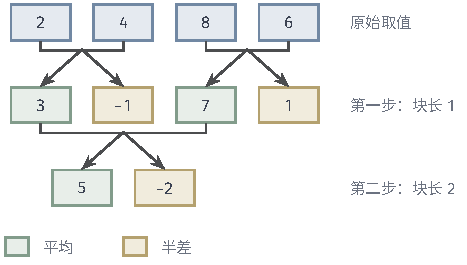
\includegraphics[width=79.07mm]{figures/04-spaces-measures-and-geometry/03-function-spaces/tikz/wavelet-average-tree/figure.pdf}
  \caption{对$(2,4,8,6)$的逐层平均与半差。蓝框是原始取值，绿框是平均，黄框是半差。每一步把一对框换成一个平均和一个半差，半差不再变动，平均进入下一步。}
  \label{fig:wavelet-average-tree}
\end{BookInlineFigure}

\paragraph{差值记录的尺度与位置}
每个半差都对应一个“块”和这一块的左右两半。细层的$-1$只比较$a_0$与$a_1$，块长为一段；粗层的$-2$比较前两段的平均$3$与后两段的平均$7$，块长为两段。块的长短给出尺度，块的位置给出位置，块越短，半差描述的变化越局部。

局部性可以直接检验。把$a_2$从$8$改成$9$，得到$(2,4,9,6)$。第一步的半差和平均变成
\[
 (2,4)\mapsto(3,-1),\qquad(9,6)\mapsto\Bigl(\frac{15}2,\frac32\Bigr).
\]
第二步对平均$(3,15/2)$再做一次，得到
\[
 \Bigl(3,\frac{15}2\Bigr)\mapsto\Bigl(\frac{21}4,-\frac94\Bigr).
\]
比较前后两组数，比较$a_0$与$a_1$的半差$-1$不变，变化的只有包含第$2$段的那些块：细层的$1$变成$3/2$，粗层的$-2$变成$-9/4$，总平均$5$变成$21/4$。一处取值的改动在每一层只影响一个系数。

\subsection{正交变换与逆变换}
\label{sec:wavelet-orthogonal-transform}

上一小节的新坐标已经能够恢复原向量，但还不是一组标准正交基下的坐标，因为它没有保持平方和。由式~\eqref{eq:wavelet-average-difference}直接计算，
\[
 s^2+d^2=\frac{(a+b)^2+(a-b)^2}{4}=\frac{a^2+b^2}{2}.
\]
每做一步，平方和减半。第~\ref{chap:function-inner-product-spaces}章的正交展开要求坐标平方和等于长度的平方，所以我们把两个新系数都乘以$\sqrt2$。

\paragraph{二阶正交变换}
把一对取值$(a,b)$换成
\begin{equation}
 \begin{bmatrix}s\\d\end{bmatrix}
 =\bm H_2\begin{bmatrix}a\\b\end{bmatrix},\qquad
 \bm H_2=\frac{1}{\sqrt2}\begin{bmatrix}1&1\\1&-1\end{bmatrix}.
 \label{eq:wavelet-h2}
\end{equation}
即$s=(a+b)/\sqrt2$，$d=(a-b)/\sqrt2$。这里沿用记号$s,d$，它们比式~\eqref{eq:wavelet-average-difference}中的量都大$\sqrt2$倍。

直接相乘可以核对
\[
 \bm H_2^{\top}\bm H_2=\frac12\begin{bmatrix}2&0\\0&2\end{bmatrix}=\bm I.
\]
所以$\bm H_2$是正交矩阵，这一步保持平方和，逆矩阵等于转置。$\bm H_2$还是对称的，于是逆变换与正变换形式相同。正交矩阵的这些性质见\BookChapterRef{chap:inner-product-spaces}{卷二第4章“内积空间”}。

\paragraph{多层变换}
对长度$N=2^J$的向量，第一层对全部$N/2$对取值作用$\bm H_2$，得到$N/2$个粗系数和$N/2$个细节系数。第二层只对粗系数两两作用$\bm H_2$，细节系数原样保留；依此类推，共做$J$层。

每一层在被处理的坐标上是若干个$\bm H_2$拼成的分块对角正交矩阵，在其余坐标上是恒等，所以每一层都是正交变换，它们的复合也是正交变换。我们把输出排成“最粗项在前，细节由粗到细”：先写最后剩下的一个粗系数，再写最粗一层的细节，最后写第一层得到的$N/2$个细节。

记这样得到的矩阵为$\bm W_N$，称$\bm c=\bm W_N\bm a$为$\bm a$的\term{Haar变换}（Haar transform）。由正交性，
\begin{equation}
 \lVert\bm c\rVert_2=\lVert\bm a\rVert_2,\qquad \bm a=\bm W_N^{\top}\bm c.
 \label{eq:wavelet-finite-haar-isometry}
\end{equation}
计算量也很小：第一层处理$N/2$对，第二层$N/4$对，总共$N-1$对。每对只做两次加减和两次乘以$1/\sqrt2$，所以运算次数与$N$成正比。

\begin{example}[四个取值的正交Haar变换]
\label{ex:wavelet-four-values-orthogonal}
仍取$\bm a=(2,4,8,6)$。第一层把两对取值分别作用$\bm H_2$：
\[
 (2,4)\mapsto(3\sqrt2,-\sqrt2),\qquad(8,6)\mapsto(7\sqrt2,\sqrt2).
\]
第二层把粗系数$(3\sqrt2,7\sqrt2)$再作用一次：
\[
 (3\sqrt2,7\sqrt2)\mapsto\Bigl(\frac{10\sqrt2}{\sqrt2},\frac{-4\sqrt2}{\sqrt2}\Bigr)=(10,-4).
\]
按约定排序，得到
\[
 \bm c=(10,-4,-\sqrt2,\sqrt2).
\]

这四个数也可以一次写成矩阵乘法：
\[
 \bm W_4=\begin{bmatrix}
 1/2&1/2&1/2&1/2\\
 1/2&1/2&-1/2&-1/2\\
 1/\sqrt2&-1/\sqrt2&0&0\\
 0&0&1/\sqrt2&-1/\sqrt2
 \end{bmatrix}.
\]
各行长度为$1$且两两正交。平方和核对如下：
\[
 4+16+64+36=120,\qquad 100+16+2+2=120.
\]

逆变换$\bm W_4^{\top}\bm c$逐分量计算，四个分量依次是
\[
 5-2-1=2,\quad5-2+1=4,\quad5+2+1=8,\quad5+2-1=6.
\]
这恢复了原向量。
\end{example}

\paragraph{矩阵的各行就是新基}
$\bm c=\bm W_4\bm a$的第$i$个分量是$\bm W_4$第$i$行与$\bm a$的点积。所以$\bm W_4$的四行组成$\mathbb R^4$的一组新标准正交基，而$\bm c$是$\bm a$在这组基下的坐标。

第一行是常数向量，读取整体水平；第二行把前后两半相减，读取最粗的起伏；后两行只在相邻两个位置非零，读取最细的局部起伏。从标准基换到这组基，向量本身没有变，变的只是读取它的方式。

\paragraph{与平均和半差的关系}
比较两个例子，对应系数之间的比例是
\[
 10=2\times5,\quad-4=2\times(-2),\quad-\sqrt2=\sqrt2\times(-1),\quad\sqrt2=\sqrt2\times1.
\]
一般地，若一个系数对应由$2^m$个原始取值组成的块，则正交变换给出的系数等于$2^{m/2}$乘以该块的平均或半差。

对$m$归纳可以验证这一点。两个长为$2^{m-1}$的子块，平均记为$s_L,s_R$，归纳假设说它们的粗系数是$2^{(m-1)/2}s_L$和$2^{(m-1)/2}s_R$。再作用$\bm H_2$，第一个分量是
\[
 \frac{2^{(m-1)/2}(s_L+s_R)}{\sqrt2}=2^{m/2}\cdot\frac{s_L+s_R}{2},
\]
这正是$2^{m/2}$乘以大块的平均，半差同理。两种算法携带相同的信息，区别只在每个系数的比例因子，正交版本用这些因子换来了长度不变。
